\chapter{Cardinalidad}

Ahora sí arranca el primer capítulo importante de la materia.

\section{Conjuntos finitos y numerables}

Como se puede esperar, la definición de conjunto finito es bastante intuitiva.

\begin{definition}
	Decimos que un conjunto $A$ es \emph{finito} si es vacío o existe una biyección $f: \llbracket n \rrbracket \to  A$. Definimos el $ \lvert A \rvert = n$ y $ \lvert \emptyset \rvert = 0$. Además, $A$ es \emph{infinito} si no es finito.
\end{definition}

Por si no lo habías visto antes, la notación $\llbracket n \rrbracket$ es el conjunto de números naturales hasta $n$.

\begin{definition}
	Decimos que $A$ es \emph{numerable} si existe una biyección $f: \mathbb{N} \to  A$. Además, si $A$ es numerable o finito decimos que es \emph{contable}.
\end{definition}

La idea detrás de armar biyecciones entre conjuntos para probar su cardinalidad se debe a que es imposible ``contar'' de manera tradicional los elementos de un conjunto.

\begin{example}
	El conjunto $\mathbb{Z}$ es numerable.
\end{example}

\begin{proof}[Solución]
	Para demostrar que $\mathbb{Z}$ es numerable, necesitamos encontrar una biyección $f : \mathbb{N} \to \mathbb{Z}$. La definimos como
	\begin{equation*}
		f(n) = \begin{cases}
			\frac{n}{2}    & \text{si } n \text{ es par},   \\
			-\frac{n-1}{2} & \text{si } n \text{ es impar}.
		\end{cases}
	\end{equation*}
	Aunque a simple vista sea difícil verlo, esta función manda a los pares a $\mathbb{N}$ y a los impares a $\mathbb{Z}_{\leq 0}$.
\end{proof}

\begin{example}
	El conjunto $\mathbb{Q}$ es numerable.
\end{example}

\begin{proof}[Solución]
	Buscamos una función $f : \mathbb{N} \to \mathbb{Q}$ biyectiva. Primero, hacemos una biyección de $\mathbb{N}$ a $\mathbb{Q}^+$. Definimos la función de la siguiente manera:
	\begin{center}
		\begin{tikzpicture}[
		scale=1.1, % Escala general
		font=\small, % Fuente para las fracciones
		node_style/.style={minimum size=2.2em, inner sep=1pt}, % Estilo para nodos de fracciones
		path_arrow/.style={->, >=stealth, thick, accentcolor, shorten >=2pt, shorten <=2pt}
	]
	% Coordenadas base para la tabla
	\def\xstart{0}
	\def\ystart{0}
	\def\xstep{1.3} % Separación horizontal
	\def\ystep{-1.2} % Separación vertical

	% Dibujar la cuadrícula de fracciones p/q (todas)
	% Fila q=1
	\node[node_style] (f-1-1) at (\xstart + 1*\xstep, \ystart + 1*\ystep) {$\frac{1}{1}$};
	\node[node_style] (f-2-1) at (\xstart + 2*\xstep, \ystart + 1*\ystep) {$\frac{2}{1}$};
	\node[node_style] (f-3-1) at (\xstart + 3*\xstep, \ystart + 1*\ystep) {$\frac{3}{1}$};
	\node[node_style] (f-4-1) at (\xstart + 4*\xstep, \ystart + 1*\ystep) {$\frac{4}{1}$};
	\node at (\xstart + 4.8*\xstep, \ystart + 1*\ystep) {$\dots$};

	% Fila q=2
	\node[node_style] (f-1-2) at (\xstart + 1*\xstep, \ystart + 2*\ystep) {$\frac{1}{2}$};
	\node[node_style] (f-2-2) at (\xstart + 2*\xstep, \ystart + 2*\ystep) {$\frac{2}{2}$};
	\node[node_style] (f-3-2) at (\xstart + 3*\xstep, \ystart + 2*\ystep) {$\frac{3}{2}$};
	\node[node_style] (f-4-2) at (\xstart + 4*\xstep, \ystart + 2*\ystep) {$\frac{4}{2}$};
	\node at (\xstart + 4.8*\xstep, \ystart + 2*\ystep) {$\dots$};

	% Fila q=3
	\node[node_style] (f-1-3) at (\xstart + 1*\xstep, \ystart + 3*\ystep) {$\frac{1}{3}$};
	\node[node_style] (f-2-3) at (\xstart + 2*\xstep, \ystart + 3*\ystep) {$\frac{2}{3}$};
	\node[node_style] (f-3-3) at (\xstart + 3*\xstep, \ystart + 3*\ystep) {$\frac{3}{3}$};
	\node[node_style] (f-4-3) at (\xstart + 4*\xstep, \ystart + 3*\ystep) {$\frac{4}{3}$};
	\node at (\xstart + 4.8*\xstep, \ystart + 3*\ystep) {$\dots$};

	% Fila q=4
	\node[node_style] (f-1-4) at (\xstart + 1*\xstep, \ystart + 4*\ystep) {$\frac{1}{4}$};
	\node[node_style] (f-2-4) at (\xstart + 2*\xstep, \ystart + 4*\ystep) {$\frac{2}{4}$};
	\node[node_style] (f-3-4) at (\xstart + 3*\xstep, \ystart + 4*\ystep) {$\frac{3}{4}$};
	\node[node_style] (f-4-4) at (\xstart + 4*\xstep, \ystart + 4*\ystep) {$\frac{4}{4}$};
	\node at (\xstart + 4.8*\xstep, \ystart + 4*\ystep) {$\dots$};

	% Puntos suspensivos verticales
	\foreach \pxval in {1,...,4}{
			\node at (\xstart + \pxval*\xstep, \ystart + 4.8*\ystep + 0.1*\ystep) {$\vdots$};
		}

	% Dibujar el camino de enumeración diagonal con flechas curvas en los "giros"

	% Diagonal 1 (p+q=2)
	% 1/1 -> (inicio de la siguiente diagonal) 2/1
	\draw[path_arrow] (f-1-1) to [out=0, in=180, looseness=0.8] (f-2-1); % Curva suave a la derecha

	% Diagonal 2 (p+q=3)
	% 2/1 -> 1/2
	\draw[path_arrow] (f-2-1) to [out=-135, in=45, looseness=0.8] (f-1-2); % Curva hacia abajo e izquierda
	% 1/2 -> (inicio de la siguiente diagonal) 3/1
	\draw[path_arrow] (f-1-2) to [out=0, in=180, looseness=0.8] (f-3-1); % Curva suave a la derecha

	% Diagonal 3 (p+q=4)
	% 3/1 -> 2/2
	\draw[path_arrow] (f-3-1) to [out=-135, in=45, looseness=0.8] (f-2-2); % Curva hacia abajo e izquierda
	% 2/2 -> 1/3
	\draw[path_arrow] (f-2-2) to [out=-135, in=45, looseness=0.8] (f-1-3); % Curva hacia abajo e izquierda
	% 1/3 -> (inicio de la siguiente diagonal) 4/1
	\draw[path_arrow] (f-1-3) to [out=0, in=180, looseness=0.8] (f-4-1); % Curva suave a la derecha

	% Diagonal 4 (p+q=5)
	% 4/1 -> 3/2
	\draw[path_arrow] (f-4-1) to [out=-135, in=45, looseness=0.8] (f-3-2); % Curva hacia abajo e izquierda
	% 3/2 -> 2/3
	\draw[path_arrow] (f-3-2) to [out=-135, in=45, looseness=0.8] (f-2-3); % Curva hacia abajo e izquierda
	% 2/3 -> 1/4
	\draw[path_arrow] (f-2-3) to [out=-135, in=45, looseness=0.8] (f-1-4); % Curva hacia abajo e izquierda

	% Nota sobre el patrón
	\node[align=center, text width=7cm, font=\scriptsize, below=0.8cm of f-1-4] at (\xstart + 2.5*\xstep, \ystart + 5.2*\ystep) {
		Patrón de recorrido diagonal de todas las fracciones $\frac{p}{q}$.
		Para $\mathbb{Q}^+$, se omiten las fracciones reducibles.
	};

\end{tikzpicture}

	\end{center}
	Se puede ver a simple vista que es biyectiva.
\end{proof}

En esencia, acá probamos que $\mathbb{N} \times \mathbb{N}$ es numerable. Es más, a continuación vamos a ver una notación muy útil.

\section{Coordinabilidad}

La idea de la notación de coordinabilidad es expresar que dos conjuntos tienen la misma cardinalidad.

\begin{definition}
	Si existe $f: A \to  B$ biyectiva, entonces se dice que $A$ y $B$ son \emph{coordinables} y lo denotamos como $A \sim B$.
\end{definition}

Notemos que por definición, todo conjunto numerable es coordinable con $\mathbb{N}$.

\begin{lemma}
	Todo subconjunto de $\mathbb{N}$ es contable.
\end{lemma}

\begin{proof}
	Si $A$ es finito, entonces ya estamos. Supongamos que $A$ es infinito. Defino la función $f: \mathbb{N} \to A$ tal que $f(1) = \min A$ y
	\begin{equation*}
		f(n+1) = \min (A \setminus \{ f(1), f(2), \dots, f(n) \}).
	\end{equation*}
	Como $A$ es infinito, $f$ está bien definida. Además, $f$ es claramente una biyección. Por lo tanto, $A$ es contable.
\end{proof}

Entonces, el conjunto de los números primos es numerable, así como $2 \mathbb{N}$.

\begin{proposition}
	Sea $X$ un conjunto \textit{numerable}. Si existe $f: X \twoheadrightarrow Y$ sobreyectiva, entonces $Y$ es contable.
\end{proposition}

\begin{proof}
	Si $X \neq \mathbb{N}$ simplemente consideramos una biyección de $\mathbb{N}$ a $X$. Entonces, podemos suponer que $X = \mathbb{N}$.

	Sea $f: X \twoheadrightarrow Y$ sobreyectiva. Definimos la función
	$$
		g: Y \to \mathbb{N} \text{ tal que } y \mapsto \min f^{-1}(y).
	$$
	La función $g$ está bien definida porque $f$ es sobreyectiva, lo que garantiza que $f^{-1}(y) \neq \emptyset$ para todo $y \in Y$. Como $g$ es inyectiva, la restricción $g|_{\operatorname{Im}g}$ es biyectiva. Dado que encontramos una biyección entre $Y$ y un subconjunto de $\mathbb{N}$, demostramos que $Y$ es contable.
\end{proof}

\begin{remark}
	Un conjunto $Y$ es contable si y sólo si existe $f : \mathbb{N} \twoheadrightarrow Y$ sobreyectiva.
\end{remark}

Ahora vamos a ver, probablemente, la proposición más útil de este capítulo.

\begin{proposition}
	La unión numerable de conjuntos numerables es numerable.
\end{proposition}

\begin{proof}
	Sea $\{ A_{n} \}_{n \in \mathbb{N}}$ una famlia de conjuntos numerables. Dado que cada $A_n$ es numerable, en particular es coordinable con $\mathbb{N} \times \{ n \}$. Por lo tanto,
	\begin{equation*}
		\bigcup_{n \in \mathbb{N}} A_n \sim \bigcup_{n \in \mathbb{N}} \mathbb{N} \times \{ n \} = \mathbb{N} \times \mathbb{N} \sim \mathbb{N}.
	\end{equation*}
	Por lo tanto, la unión numerable de conjuntos numerables es numerable.
\end{proof}

\begin{example}
	El conjunto de los polinomio con coeficientes racionales $\mathbb{Q}[x]$ es numerable.
\end{example}

\begin{proof}[Solución]
	Veamos que $\mathbb{Q}[x]$ es numerable. Recordemos que un polinomio es de la forma
	\begin{equation*}
		a_{n} x^n + a_{n-1} x^{n-1} + \dots + a_{1} x + a_0,
	\end{equation*}
	donde $a_0, a_1, \ldots, a_n \in \mathbb{Q}$ y $n \in \mathbb{N}_0$. Por lo tanto, podemos pensar un polinomio como
	\begin{equation*}
		(a_0, a_1, \ldots, a_n) \in \mathbb{Q}^{n+1}.
	\end{equation*}
	Entonces,
	\begin{equation*}
		\mathbb{Q}[x] \sim \bigcup_{n \in \mathbb{N}_0} \mathbb{Q}^{n+1}
	\end{equation*}
	y como $\mathbb{Q}^n$ es numerable para todo $n \in \mathbb{N}$, $\mathbb{Q}[x]$ es numerable.
\end{proof}

Notemos que omití algunos detalles en la demostración. Por ejemplo, la asociación que dí no es exactamente una biyección, ya que $a_n \neq 0$. Pero no es tan dramático el problema, simplemente con saber que $\mathbb{Q} \setminus \left\{ 0 \right\} \sim \mathbb{Q}$, entonces podemos encontrar la biyección.


\section{Conjuntos no numerables}

El primer conjunto no numerable que vamos a ver es $\mathbb{R}$.

\begin{proposition}
	El conjunto de los numeros reales no es numerable.
\end{proposition}

\begin{proof}[Solución]
	Para facilitarnos la vida, podemos considerar la biyección $g: \mathbb{R} \to (0, 1)$ dada por $g(x) = \frac{\tan^{-1} (x)}{\pi} + \frac{1}{2}$.
	\begin{center}
		\color{red} INSERTAR GRÁFICO
	\end{center}
	Esto da una biyección entre $\mathbb{R}$ y $(0, 1)$. Por lo tanto, basta con demostrar que no existe una biyección entre $\mathbb{N}$ y $(0, 1)$ para ver que $\mathbb{R}$ no es cordinable con $\mathbb{N}$.

	Supongamos que $\mathbb{N}$ es coordinable con $(0, 1)$. Sea $f: \mathbb{N} \to (0, 1)$ una biyección tal que
	\begin{align*}
		f(1) & = 0.\textcolor{accentcolor}{a_{11}} a_{12}a_{13}\dots \\
		f(2) & = 0.a_{21}\textcolor{accentcolor}{a_{22}}a_{23}\dots  \\
		f(3) & = 0.a_{31}a_{32}\color{accentcolor}{a_{33}}\dots      \\
		     & \dots
	\end{align*}
	Consideramos el número definido por agarrar los dígitos de la diagonal y sumarle $1$ si es menor que $9$ o restarle $1$ si es $9$. Nos queda el número
	$$
		0.a'_{11}a'_{22}a'_{33}\dots
	$$
	Este número es distinto a $f(n)$ en el $n$-ésimo dígito decimal. Lo cual es absurdo, ya que si $f$ es biyectiva debería existir un natural $m$ tal que $f(m) = 0.a'_{11}a'_{22}a'_{33}\dots$. Por lo tanto, demostramos que $\mathbb{N}$ no es coordinable con $\mathbb{R}$.
\end{proof}

Aclaro una pequeña notación. Cuando escribimos $Y^X$ nos referimos al conjunto de funciones de $X$ a $Y$:
\begin{equation*}
	Y^{X} = \left\{ f : X \to Y \right\}.
\end{equation*}

\begin{proposition}
	El conjunto partes $\mathcal{P}(X)$ es coordinable con $2^X$.
\end{proposition}

\begin{proof}
	Definimos la función $f : \mathcal{P}(X) \to \{0, 1\}^X$ como
	\begin{equation*}
		A \subseteq X \mapsto g_A,
	\end{equation*}
	donde $g_A : X \to \{ 0, 1 \}$ tal que
	\begin{equation*}
		g_A(x) = \begin{cases}
			1, & \text{ si }x \in A      \\
			0, & \text{ si } x \not\in A
		\end{cases}.
	\end{equation*}
	Esta función claramente es bitectiva.
\end{proof}

Ahora vamos a ver el Teorema de Cantor.

\begin{theorem}
	Ningún conjunto es coordinable con su conjunto de partes.
\end{theorem}

\begin{proof}
	Sea $X$ un conjunto. Queremos ver que no es coordinable con $\mathcal{P}(X)$. Supongamos que existe una biyección $f : X \to \mathcal{P}(X)$. Consideremos al siguiente subconjunto:
	\begin{equation*}
		A = \{ x \in X \mid x \not \in f(x) \}.
	\end{equation*}
	La idea de este subconjunto es forzar a que sea distinto a cada elemento de la imagen de $f$. Por lo tanto, para todo $x \in X$, $A \neq f(x)$ ya que $A$ siempre tiene un elemento que no pertenece a $f(x)$, en particular $x$. Acabamos de probar que $f$ no es sobreyectiva, por lo tanto no es biyectiva y entonces $X$ y $\mathcal{P}(X)$ no son coordinables.
\end{proof}


\section{Cardinales y Axioma de Elección}

En estas notas (y en la cursada) se acepta el axioma de elección y el principio de buena ordenación. El axioma de elección postula lo siguiente.

\begin{axiom}[Axioma de elección]
	Sea $\mathcal{F}$ una familia de conjuntos no vacíos y disjuntos dos a dos. Entonces, existe una función $f: \mathcal{F} \to \bigcup \mathcal{F}$ tal que $f(A) \in A$ para todo $A \in \mathcal{F}$.
\end{axiom}

Otras formulaciones equivalentes son:

\begin{enumerate}[label=(\roman*)]
	\item Sea $X$ un conjunto. Existe una función
	      $$f: \mathcal{P}(X) - \{ \emptyset \} \to X$$
	      tal que $f(A) \in A$ para todo $A \in \mathcal{P}(X)$.
	\item El producto cartesiano de conjuntos no vacíos es no\\ vacío.
\end{enumerate}

El axioma de elección también es equivalente al principio de buena ordenación.

\begin{axiom}[Principio de buena ordenación]
	Todo conjunto puede ser dotado de un orden tal que todo subconjunto no vacío tiene un elemento mínimo. A este tipo de orden se le llama \textit{orden bueno}.
\end{axiom}

Aceptando el axioma de elección (y en consecuencia el principio de buen ordenamiento) se puede demostrar el lema de Zorn.

\begin{axiom}[Lema de Zorn]
	Son equivalentes:
	\begin{enumerate}
		\item Sea $(A, \preceq)$ un conjunto parcialmente ordenado tal que toda cadena de $A$ tiene cota superior. Entonces, $A$ tiene un elemento maximal.
		\item Sea $(A, \preceq)$ un conjunto parcialmente ordenado tal que toda cadena de $A$ tiene supremo. Entonces, $A$ tiene un elemento maximal.
		\item Todo conjunto parcialmente ordenado tiene una cadena maximal.
	\end{enumerate}
\end{axiom}

Ahora sí, veamos un teorema que vamos a usar bastante.

\begin{theorem}
	Sean $f: X \hookrightarrow Y$ y $g: Y \hookrightarrow X$ funciones \textit{inyectivas}. Entonces, existe una biyección $h: X \to  Y$.
\end{theorem}

\begin{proof}
	La idea detrás de esta demostración es particionar a los conjuntos $X$ e $Y$ en $A$, $B$ y $A'$, $B'$, respectivamente, de forma tal que
	$$
		A \cap B = A' \cap B' = \emptyset,
	$$
	y
	$$
		A \cup B = X \quad \text{y} \quad A' \cup B' = Y,
	$$
	y además
	$$
		f(A) = A' \quad \text{y} \quad f(B) = B'.
	$$
	\begin{center}
		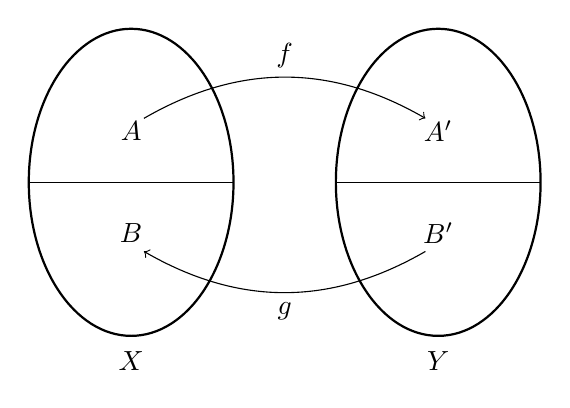
\begin{tikzpicture}[scale=0.65]
	% Sets X and Y
	\draw[thick] (0,0) ellipse (2 and 3);
	\draw[thick] (6,0) ellipse (2 and 3);

	% Labels for X and Y
	\node at (0,-3.5) {$X$};
	\node at (6,-3.5) {$Y$};

	% Subsets A and B in X
	\node at (0,1) {$A$};
	\node at (0,-1) {$B$};

	% Subsets A' and B' in Y
	\node at (6,1) {$A'$};
	\node at (6,-1) {$B'$};

	% Diagonal line between X and Y
	\draw (-2, 0) -- (2, 0);
	\draw (4, 0) -- (8, 0);

	\draw[-to, bend left] (0.25,1.25) to node[midway, above] {$f$} (5.75,1.25);
	\draw[-to, bend left] (5.75,-1.35) to node[midway, below] {$g$} (0.25,-1.35);
\end{tikzpicture}


	\end{center}

	Esto se reduce a encontrar $A \subseteq X$ tal que
	$$
		X - g(Y - f(A)) = A.
	$$
	Definimos $\Phi : \mathcal{P}(X) \to  \mathcal{P}(X)$ tal que $\Phi(A) = X - g(Y - f(A))$. Lo cual nos da la siguiente ecuación,
	$$
		\Phi (A) = A.
	$$
	Veamos que $\Phi$ es un morfismo de orden con en $(\mathcal{P}(X), \subseteq )$. Sean $X_{0}$ y $X_{1}$ subconjuntos de $X$. Supongamos que $X_{0} \subseteq X_{1}$. Entonces,
	\begin{align*}
		X_{0}               & \subseteq X_{1}               \\
		f(X_{0})            & \subseteq f(X_{1})            \\
		Y - f(X_{0})        & \supseteq Y - f(X_{1})        \\
		g(Y - f(X_{0}))     & \supseteq g(Y - f(X_{1}))     \\
		X - g(Y - f(X_{0})) & \subseteq X - g(Y - f(X_{1})) \\
		\Phi(X_{0})         & \subseteq \Phi(X_{1})
	\end{align*}
	probando que $\Phi$ es un morfismo de orden. Y como ya sabemos, $(\mathcal{P}(X), \subseteq)$ es un reticulado completo. Por lo tanto, podemos utilizar el teorema del punto fijo, dándonos un $A \subseteq X$ tal que $\Phi (A) = A$.
\end{proof}

Cuando trabajamos con cardinales de conjuntos, para probar que dos conjuntos tienen el mismo cardinal es necesario establecer una biyección o inyecciones hacia ambos lados. Sin embargo, encontrar la función en particular puede ser molesto a veces. Para esto sirve la aritmética de cardinales. Nos ahorra el trabajo de encontrar una función en particular y nos permite trabajar con cardinales generales.

\begin{definition}
	Decimos que dos conjuntos $A$ y $B$ tienen el mismo \emph{cardinal} si existe una función biyectiva $f: A \to  B$ y lo denotamos como $\lvert A \rvert = \lvert B \rvert$.
\end{definition}

Por ejemplo, si $A$ es un conjunto numerable, entonces
$$
	\lvert A \rvert = \lvert \mathbb{N} \rvert.
$$
En general, como hay algunos cardinales que son más ocurrentes, los denotamos de una forma especial.

\begin{definition}
	Denotamos
	\begin{itemize}
		\item El cardinal de $\mathbb{N}$ como $\aleph_0$.
		\item El cardinal de $\mathbb{R}$ como $\mathfrak{c}$.
	\end{itemize}
\end{definition}

\begin{remark}
	Si $A$ es numerable, entonces su cardinal es $\aleph_0$.
\end{remark}

\begin{definition}
	Sean $A$ y $B$ conjuntos. Si existe una función inyectiva $f: A \hookrightarrow B$, entonces $\lvert A \rvert \leq \lvert B \rvert$.
\end{definition}

Si bien tratamos con funciones inyectivas, podríamos haber utilizado funciones sobreyectivas para las definiciones; ya que, si existe $f: A \hookrightarrow B$ inyectiva y $A \neq \emptyset $, entonces existe $g: B \twoheadrightarrow A$ sobreyectiva.

A continuación veremos una suerte de tricotomía pero para los cardinales. Para la demostración de este teorema, es necesario el lema de Zorn.

\begin{theorem}
	Sean $X$ e $Y$ conjuntos no vacíos. Existe $f: X \hookrightarrow Y$ inyectiva o existe $g: Y \hookrightarrow X$ inyectiva.
\end{theorem}

\begin{proof}
	Consideramos el conjunto ordenado
	$$
		\mathcal{A} = \{ (A, f_{A}) \mid f_{A}: A \subseteq X \hookrightarrow Y  \text{ es inyectiva}\}
	$$
	con el orden $(A, f_{A}) \preceq (B, f_{B})$ si $A \subseteq B$ y $f_{B}|_{A} = f_{A}$. Queremos utilizar el lema de Zorn, para eso necesitamos probar que toda cadena de $\mathcal{A}$ tiene cota superior.

	Sea $\mathcal{C} = \{ (A_{i}, f_{A_{i}})\}_{i \in I}$ una cadena de $\mathcal{A}$. Consideremos el par $(A, f_{A})$ donde
	$$
		A = \bigcup_{i \in I} A_{i}
	$$
	y
	$$
		f_{A} : A \to Y \text{ donde } f_{A}(a) = f_{A_{i}}(a) \text{ si } a \in A_{i}.
	$$
	Es evidente que $(A_{i}, f_{A_{i}}) \preceq (A, f_{A})$ para todo $i \in I$.

	Probemos que $f_{A}$ está bien definida ya que, para cualesquiera $A_{i}, A_{j}$ de $\mathcal{C}$ tales que $A_{i} \subseteq A_{j}$ (sin pérdida de generalidad), $f_{A_{j}|_{A_{i}} = f_{A_{i}}}$.

	Veamos que $A \in \mathcal{A}$. Claramente $A \subseteq X$. Probemos que $f_{A}$ es inyectiva. Sean $a, a' \in A$ tales que $f_{A}(a) = f_{A}(a')$. Entonces, existe un $i \in I$ tal que $a, a' \in A_{i}$, ya que $\mathcal{C}$ es una cadena. Por lo tanto, obtenemos
	$$
		f_{A_{i}}(a) =f_{A_{i}}(a'),
	$$
	y por inyectividad de $f_{A_{i}}$, $a = a'$. Lo cual prueba que $f_{A}$ es inyectiva. Entonces, como $A \in \mathcal{A}$, tenemos que $\mathcal{C}$ está acotado superiormente.

	Como toda cadena de $\mathcal{A}$ está acotada superiormente, por el lema de Zorn, existe un elemento maximal. Sea $(B, f_{B})$ un elemento maximal. Necesariamente, $\operatorname{dom} f_{B} = X$ o
	$\operatorname{Im} Y$, del caso contrario $(B, f_{B})$ no sería maximal. Si $\operatorname{dom} f_{B} = X$, ya conseguimos nuestra función inyectiva. Si $\operatorname{Im} Y$, entonces definimos $f: Y \hookrightarrow X$ donde $f(y) = f_{B}^{-1}(y)$.
\end{proof}

\begin{remark}
	Esto es equivalente a decir que, para dos conjuntos $X$ e $Y$ cualesquiera, $\lvert X \rvert \leq \lvert Y \rvert$ o $\lvert X \rvert \geq \lvert Y \rvert$.
\end{remark}

\begin{proposition}
	Sea $A$ un conjunto \textit{infinito}. Entonces, existe una partición de $A$ tal que todas las partes son numerables. Es decir,
	$$
		A = \bigsqcup_{i \in I} A_i,
	$$
	donde $A_i$ es numerable para todo $i \in I$.
\end{proposition}

\begin{proof}
	{\color{red} La demostración de esta proposición no la incluyo.}
\end{proof}

Volviendo a los cardinales.

\begin{definition}
	Sean $A$ y $B$ conjuntos disjuntos (por praciticidad). Si $a = \lvert A \rvert$ y $b = \lvert B \rvert$, entonces
	\begin{itemize}
		\item $a + b = |A \cup B|$.
		\item $a \cdot b = |A \times B|$.
		\item $a^{b} = |A^{B}|$.
	\end{itemize}
\end{definition}

Podemos operar como lo esperaríamos.

\begin{proposition}
	Sean $a, b, c$ cardinales. Entonces:
	\begin{itemize}
		\item $a + b = b + a$.
		\item $a \cdot b = b \cdot a$.
		\item $(a + b) + c = a + (b + c)$.
		\item $(a \cdot b) \cdot c = a \cdot (b \cdot c)$.
		\item $a \cdot (b + c) = a \cdot b + a \cdot c$.
		\item $a^{b+c} = a^{b} \cdot a^{c}$.
		\item $a^{b^{c}} = a^{b \cdot c}$.
	\end{itemize}
\end{proposition}

\begin{proof}
	Las propiedades se deducen directamente de las definiciones de suma y producto de cardinales, utilizando las propiedades correspondientes de las uniones disjuntas y los productos cartesianos de conjuntos.
\end{proof}
